%%%%%%%%%%%%%%%%%%%%%%%%%%%%%%%%%%%%%%%%%
% Tufte Essay
% LaTeX Template
% Version 2.0 (19/1/19)
%
% This template originates from:
% http://www.LaTeXTemplates.com
%
% Authors:
% The Tufte-LaTeX Developers (https://www.ctan.org/pkg/tufte-latex)
% Vel (vel@LaTeXTemplates.com)
%
% License:
% Apache License, version 2.0
%
%%%%%%%%%%%%%%%%%%%%%%%%%%%%%%%%%%%%%%%%%

%----------------------------------------------------------------------------------------
%	PACKAGES AND OTHER DOCUMENT CONFIGURATIONS
%----------------------------------------------------------------------------------------

\documentclass{tufte-handout} % Use A4 paper by default, remove 'a4paper' for US letter

\usepackage{graphicx} % Required for including images
\setkeys{Gin}{width=\linewidth, totalheight=\textheight, keepaspectratio} % Default images settings
\graphicspath{{Figures/}{./}} % Specifies where to look for included images (trailing slash required)

\usepackage{booktabs} % Required for better horizontal rules in tables

\usepackage{subfiles}

\usepackage{pgfplots}
\pgfplotsset{compat=1.18}

%----------------------------------------------------------------------------------------
%	TITLE SECTION
%----------------------------------------------------------------------------------------

\title{Algebraic and Transcendental functions}

\author{Professor: Francisco Vazquez-Tavares}

\date{Last compilation: \today} % Date, use \date{} for no date


%----------------------------------------------------------------------------------------
%	COMMANDS SECTION
%----------------------------------------------------------------------------------------


%----------------------------------------------------------------------------------------

\begin{document}

\maketitle % Print the title section

%----------------------------------------------------------------------------------------
%	ABSTRACT/SUMMARY
%----------------------------------------------------------------------------------------

\begin{abstract}
    \textbf{\large Name: }\hfill November 18, 2025
\end{abstract}

%----------------------------------------------------------------------------------------
%	ESSAY BODY
%----------------------------------------------------------------------------------------


\marginpar{
    {\bfseries\Large Algebra Toolkit}

    {\bfseries\large Algebra properties}
    \begin{gather*}
        a+b = b+a, \\
        \qty(a+b)+c = a+\qty(b+c), \\
        a\qty(b+c) = ab+ac, \\
        \frac{a}{b} + \frac{c}{d} = \frac{ad+bc}{bd}, \quad
        \frac{a}{b} \cdot \frac{c}{d} = \frac{ac}{bd}, \\
        \frac{-a}{b} = -\frac{a}{b} = \frac{a}{-b}, \\
        \frac{\frac{a}{b}}{\frac{c}{d}} = \frac{ad}{bc}
        \\
        \sqrt{ab} = \sqrt{a}\sqrt{b},\quad
        \sqrt{\frac{a}{b}} = \frac{\sqrt{a}}{\sqrt{b}},\quad
        \sqrt[n]{a} = a^{1/n}
        \\
        x=\frac{-b\pm\sqrt{b^2-4ac}}{2a},\\
        a^2-b^2 = \qty(a-b)\qty(a+b)
    \end{gather*}
    
    {\bfseries\large Laws of exponents}
    \begin{align*}
        a^r\cdot a^s = a^{r+s}, \quad & \qty(a^r)^s = a^{rs} \\
        \frac{a^r}{a^s} = a^{r-s}, \quad & \qty(ab)^r = a^r b^r \\
        \qty(\frac{a}{b})^r = \frac{a^r}{b^r},\quad & b\neq 0
    \end{align*}

    {\bfseries\large Laws of Logarithms}
    \begin{align*}
        \log_a\qty(AB) &= \log_a\qty(A) + \log_a\qty(B) \\
        \log_a\qty(\frac{A}{B}) &= \log_a\qty(A) - \log_a\qty(B) \\
        \log_a\qty(A^C) &= C\log_a\qty(A)
    \end{align*}

    {\bfseries\large Inverse functions property}
    \begin{gather*}
        \qty(f\circ f^{-1})(x) = x = \qty(f^{-1}\circ f)(x) \\
        \log_a(a^x) = x = a^{\log_a(x)}
    \end{gather*}
}

\section{Algebra skills}

\begin{enumerate}
    \item Use the base change formula to find the numeric value of $\log_2\qty(e^2)$ without using calculator.
    \item For the functions $f(x) = \frac{5x}{x^2+2}$ and $g(x)=\frac{1}{x}$ find the indicates composition and reduce the expressions as much as possible,
        \begin{itemize}
            \item $\qty(g\circ f)(x)$
            \item $\qty(g\circ g)(x)$ 
            \item $\qty(f\circ g)(x)$
            \item $\qty(f\circ f)(x)$
        \end{itemize}
\end{enumerate}

Use logarithmic properties to condence the following expression $2\log_{8}\qty(y) + \frac{1}{3}\left[\log_{8}\qty(x)-2\log_{8}\qty(w)\right]$.

\section{Function analysis}

Find the inverse function of $f(x)=\frac{2x-4}{4x^2+2x-10}$. 
Reduce the expression as much as possible and proof your answer by evaluation the function composition $(f\circ f^{-1})(x)=x$.



\section{Modelling with math}

\paragraph{Exponential decay} The half-life of Radium-266 is 1600 years. 
Suppose that there is a sample of \SI{1}{\kilo\gram}. 
Recalling that the mass decays exponentially, fulfill the following points.
\begin{enumerate}
    \item Write the function that models the remaining mass after t years.
    \item How much mass will remain after 4000 years?
    \item How much time will it take for the sample to be a third of its original value.
\end{enumerate}



\newpage

\section{Conic sections}
\marginpar{
    {\bfseries\Large Conic Sections}

    {\large Standard form of a circle}
    \begin{gather*}
        (x-h)^2 + (y-k)^2 = r^2
    \end{gather*}

    {\large Standard form of a parabola}
    \begin{gather*}
        (x-h) = 4a(y-k)^2,~\mathrm{or}~(y-k) = 4a(x-h)^2
    \end{gather*}

    {\large Standard form of an ellipse}
    \begin{gather*}
        \frac{(x-h)^2}{a^2} + \frac{(y-k)^2}{b^2} =1
    \end{gather*}

    {\large Standard form of a hyperbola}
    \begin{gather*}
        \frac{(x-h)^2}{a^2} - \frac{(y-k)^2}{b^2} =1
    \end{gather*}

}

\paragraph{General formula} Identify the conic section give the following general equation $16x^2-9y^2-96x-56y-81=0$.

\paragraph{Graph} Graph the following conic section $(x+5) = 0.5(y-5)^2$.

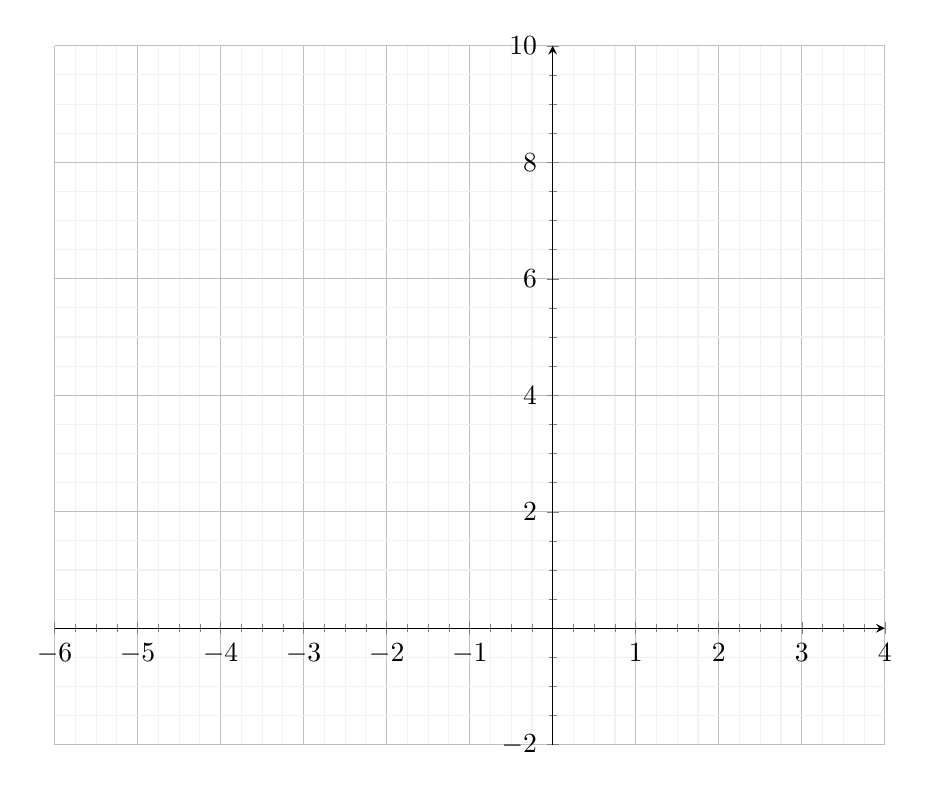
\begin{tikzpicture}
\begin{axis}[
    xmin=-6, xmax=4,
    ymin=-2, ymax=10,
    grid=both,
    minor grid style={gray!10},  % Style for minor grid lines
    minor tick num=3,
    width=\textwidth,
    axis lines=center
]
% The axis environment automatically draws the grid based on the ticks
\end{axis}
\end{tikzpicture}


\end{document}
